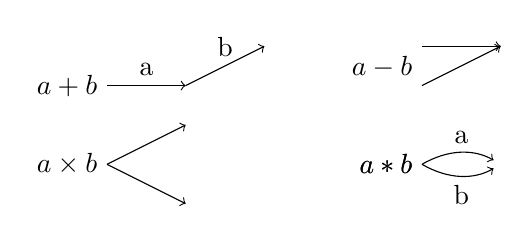
\begin{tikzpicture}[->]
\draw (0,0) node [anchor=east] {$a+b$} to node[anchor=south] {a} (1,0);
\draw (1,0) to node[anchor=south] {b} (2,0.5);

\draw (4,0.5) node [anchor=north east] {$a-b$} to (5,0.5);
\draw (4,0) to (5,0.5);

\draw (0,-1) node [anchor=east] {$a\times b$} to (1,-0.5);
\draw (0,-1) to (1,-1.5);

\draw[shorten >= 3] (4,-1) node [anchor=east] {$a*b$} to [bend left] node[anchor=south] {a} (5,-1);
\draw[shorten >= 3] (4,-1) node [anchor=east] {$a*b$} to [bend right] node[anchor=north] {b} (5,-1);
\end{tikzpicture}